%%%%%%%%%%%%%%%%%%%%%%%%%%%%%%%%%%%%%%%%%
% Developer CV
% LaTeX Template
% Version 1.0 (28/1/19)
%
% This template originates from:
% http://www.LaTeXTemplates.com
%
% Authors:
% Jan Vorisek (jan@vorisek.me)
% Based on a template by Jan Küster (info@jankuester.com)
% Modified for LaTeX Templates by Vel (vel@LaTeXTemplates.com)
%
% License:
% The MIT License (see included LICENSE file)
%
%%%%%%%%%%%%%%%%%%%%%%%%%%%%%%%%%%%%%%%%%

%----------------------------------------------------------------------------------------
%	PACKAGES AND OTHER DOCUMENT CONFIGURATIONS
%----------------------------------------------------------------------------------------

\documentclass[9pt]{developercv} % Default font size, values from 8-12pt are recommended

%----------------------------------------------------------------------------------------

\begin{document}

%----------------------------------------------------------------------------------------
%	TITLE AND CONTACT INFORMATION
%----------------------------------------------------------------------------------------

\begin{minipage}[t]{0.375\textwidth} % 45% of the page width for name
	\vspace{-\baselineskip} % Required for vertically aligning minipages
	
	% If your name is very short, use just one of the lines below
	% If your name is very long, reduce the font size or make the minipage wider and reduce the others proportionately
	\colorbox{black}{{\HUGE\textcolor{white}{\textbf{\MakeUppercase{Simone}}}}} % First name
	
	\colorbox{black}{{\HUGE\textcolor{white}{\textbf{\MakeUppercase{Rigoni}}}}} % Last name
	
	\vspace{6pt}
	
	{\huge Technical Consultant} % Career or current job title
\end{minipage}
\begin{minipage}[t]{0.225\textwidth} % 27.5% of the page width for the first row of icons
	\vspace{-\baselineskip} % Required for vertically aligning minipages
	
	% The first parameter is the FontAwesome icon name, the second is the box size and the third is the text
	% Other icons can be found by referring to fontawesome.pdf (supplied with the template) and using the word after \fa in the command for the icon you want
	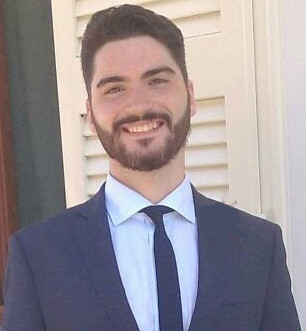
\includegraphics[width=3cm]{image_1}
\end{minipage}
\begin{minipage}[t]{0.300\textwidth} % 27.5% of the page width for the second row of icons
	\vspace{-\baselineskip} % Required for vertically aligning minipages
	
	% The first parameter is the FontAwesome icon name, the second is the box size and the third is the text
	% Other icons can be found by referring to fontawesome.pdf (supplied with the template) and using the word after \fa in the command for the icon you want
	\icon{MapMarker}{10}{Pavia, Lombardy, Italy}\\
	\icon{Phone}{10}{+39}\\
	\icon{At}{10}{\href{mailto:simone.rigoni01@gmail.com}{simone.rigoni01@gmail.com}}\\	
	\icon{Medium}{10}{\href{https://medium.com/@simone.rigoni01}{medium.com/@simone.rigoni01}}\\
	\icon{Github}{10}{\href{https://github.com/simonerigoni}{github.com/simonerigoni}}\\
	\icon{Linkedin}{10}{\href{https://www.linkedin.com/in/simone-rigoni-852b40101}{linkedin.com/in/simone-rigoni-852b40101}}\\
	\icon{Globe}{10}{\href{http://www.simonerigoni.net}{simonerigoni.net}}\\
\end{minipage}

%\vspace{0.5cm}

%----------------------------------------------------------------------------------------
%	INTRODUCTION, SKILLS AND TECHNOLOGIES
%----------------------------------------------------------------------------------------

\cvsect{Who Am I?}

\begin{minipage}[t]{0.5\textwidth} % 40% of the page width for the introduction text
	\vspace{-\baselineskip} % Required for vertically aligning minipages
	
	I graduated in Computer Engineering - Embedded and Control Systems at the University of Pavia in 2017. During my Erasmus Traineeship in Dublin I worked as Software Developer at \underline{\href{https://iot.taoglas.com/}{Firmwave}}, a young company specialized in the design of low-power hardware for IoT. I took part in the design and implementation of new features in both the bootloader and the application using C. I got passionate about Python and how to use data to solve problems so I decided to completely change my working field approaching Data Science. I started working in 2017 as Technical Consultant at Aptos which provides tools to retail enterprises to deliver omni-channel shopping experiences to customers. In 2019 I graduated from the Udacity Data Scientist Nanodegree Program. I write about Machine Learning and Data Science topics on \underline{\href{https://medium.com/@simone.rigoni01}{Medium}} and I have recently built my website \underline{\href{http://www.simonerigoni.net}{simonerigoni.net}} as a common platform for my projects
\end{minipage}
\hfill % Whitespace between
\begin{minipage}[t]{0.4\textwidth} % 50% of the page for the skills bar chart
	\vspace{-\baselineskip} % Required for vertically aligning minipages
	\begin{barchart}{5.5}
		\baritem{Python}{90}
		\baritem{SQL}{85}
		\baritem{C}{70}
		\baritem{MATLAB}{40}
		\baritem{HTML/CSS}{40}
		\baritem{MIPS}{40}
		\baritem{VBA}{40}
		%\baritem{PHP}{20}
		\baritem{Java}{20}
		\baritem{C++}{20}
	\end{barchart}
\end{minipage}

\begin{center}
	\bubbles{5/Visual Studio
		, 4/Git
		, 4/Office
		, 5/SSMS
		, 3/Spark
		, 3/AD Inventor
		, 4/TFS
		%, 4/LTSpice
		, 3/PowerBI
		, 3/Jira}
\end{center}

%----------------------------------------------------------------------------------------
%	EXPERIENCE
%----------------------------------------------------------------------------------------

\cvsect{Experience}

\begin{entrylist}
	\entry
		{10/2017 -- Currently}
		{Technical Consultant}
		{Aptos}
		{I develop T-SQL functionalities on Microsoft SQL Server (Database Engine and Analysis Services) using Management Studio, Profiler, Visual Studio and Team Foundation Server to import, process and export data to fulfill the steps of retail process such as Merchandise and Financial Planning, Assortment Plan, Forecast and Store Replenishment. Performances are a key aspect of my work because of the high volume of data used by these business process. I have been involved also in the recruiting phase for the technical interviews and in the tutoring of new hires}
		{}
		{}
		%\texttt{T-SQL}\slashsep\texttt{VBA}\slashsep\texttt{MDX}\slashsep\texttt{MDX}}
	\entry
		{06/2017 -- 12/2017}
		{Waiter}
		{Corrado Calza Food \& Co.}
		{While studying I worked as waiter for fashion events like catering for boutiques and fashion shows}
		{}
		{}
	\entry
		{09/2015 -- 07/2017}
		{Tutor}
		{Plinio Fraccaro College}
		{Tutoring regarding Computer Science and C programming for my fellow students of the college}
		{}
		{}
	\entry
		{03/2016 -- 06/2016}
		{Software Developer}
		{Firmwave}
		{During my Erasmus Traineeship with Firmwave I took part in the design and implementation of Over-the-Air programming (OTA) on a device based on STM32F4 MCU (equipped with ARM Cortex M4), implementing new features both in the bootloader and in the application, so that it could download updates from remote servers and reprogram itself. The code was written in C, with an open source toolchain based on GCC ARM + Eclipse + OpenOCD. I also took part in the development of Python based scripts for automated testing purposes}
		{}
		{}
%	\entry
%		{06/2009 -- 09/2009}
%		{Intern}
%		{Aglietta Mario - IT and office}
%		{I worked with IT technicians to provide customer support}
%		{}
%		{}
\end{entrylist}

%----------------------------------------------------------------------------------------
%	EDUCATION
%----------------------------------------------------------------------------------------

\cvsect{Education}

\begin{entrylist}
	\entry
		{10/2014 -- 10/2017}
		{Master's Degree (LM-32) in Computer Engineering - Embedded and Control Systems}
		{University of Pavia}
		{The degree program includes courses in electrical engineering, electrical drives and automation, advanced control systems, industrial automation, process control, robotics, embedded systems. The lessons, held in English, are complemented by laboratories activities, seminars and tutorials}
		{100/110}
		{Thesis: Design and implementation of a Bluetooth based indoor localization system for the sport domain}
	\entry
		{09/2011 -- 12/2014}
		{Bachelor’s Degree (L-8) in Computer Engineering}
		{University of Pavia}
		{The degree course covers various fields such as mathematics, physics, information technology, automation, electromagnetism, electronics and telecommunications}
		{95/110}
		{Thesis: Stable stationary flight of a quadcopter}
	\entry
		{09/2007 -- 07/2011}
		{Diploma ITIS - Informatics and Telecommunications}
		{ITIS Enrico Fermi of Mantova}
		{The course provides basic knowledge in computer science and electronics, in order to develop the skills necessary to analyze, size, manage and design small systems for process data}
		{73/110}
		{Thesis: On line management of an electronics store}
\end{entrylist}

%----------------------------------------------------------------------------------------
%	OTHER ACTIVITIES
%----------------------------------------------------------------------------------------

\cvsect{Other activities}

\begin{entrylist}
	\entry
		{01/2019 -- 10/2019}
		{Data Scientist Nanodegree}
		{Udacity}
		{The Data Scientist Nanodegree program is an advanced course designed to prepare the student for data scientist jobs. The topics covered were Supervised Learning, Deep Learning, Unsupervised Learning, Data storytelling, Software development and Recommendation Engines. All the theoretical lessons were followed by quiz and projects that can be found on \underline{\href{https://github.com/simonerigoni/udacity/tree/master/data_scientist_nanodegree}{Github}}}
		{}
		{Capstone Project: \underline{\href{https://towardsdatascience.com/user-churn-prediction-using-spark-22ff8dafb5c}{User churn prediction using Spark}}}
	\entry
		{06/2019 -- Currently}
		{Content Writer}
		{Medium}
		{I started writing for Medium through the Data Scientist Nanodegree and got passionate about it. I usually publish my stories on Towards Data Science and Analytics Vidhya which are some of the biggest platforms for data science topics. All my stories can be found on \underline{\href{https://medium.com/@simone.rigoni01}{Medium}} and on my website \underline{\href{http://www.simonerigoni.net}{simonerigoni.net}} is possible to interact with some of the projects I have written about. One of the latest project I made: \underline{\href{https://towardsdatascience.com/do-you-want-to-move-to-milan-neighborhoods-sentiment-analysis-using-airbnb-data-72db72ebc070}{"Do you want to move to Milan? Neighborhoods Sentiment Analysis using Airbnb data"}}}
		{}
		{}
	\entry
		{09/2016 -- 07/2017}
		{Conference organizer}
		{Plinio Fraccaro College}
		{I was coordinating the organization of conferences and others cultural events. Beside the planning activity I helped promoting the events through local newspapers and social media. I was also one of the main promoters of multidisciplinary conference "Artificial Intelligence techniques, applications and problems" which was designed to introduce and look at artificial intelligence from the point of view of various disciplines such as engineering, philosophy, law and computational linguistics}
		{}
		{}
	\entry
		{09/2018 -- 09/2018}
		{Publication: A Comparison of RSSI Filtering Techniques for Range-based Localization}
		{IEEE}
		{Received Signal Strength Indication (RSSI) is commonly used to provide distance estimates in range-based localization. Usually the localization systems use RSS at short range and RSS alongside other techniques such as Time of Flight (ToF) where the distance estimates are less reliable. For more information \underline{\href{https://ieeexplore.ieee.org/abstract/document/8502556}{IEEE Explore}}}
		{}
		{}
%	\entry
%		{03/2018 -- 03/2018}
%		{Participant}
%		{University2Business}
%		{Smart Distribution Pack Management contest organized by University2Business in collaboration with TXT e-solutions. The contest required to identify a method to optimize the process of retail distribution of textile products, with the application to a specific case. Together with a a friend, we developed a MySQL database and MATLAB scripts to manipulate data. The goal was to increase the efficiency of the existing system by creating pre-packaged packs containing products of various sizes to be sent to stores}
%		{}
%		{}
%	\entry
%		{04/2016 -- 04/2016}
%		{Participant}
%		{Dublin Airport Hackathon}
%		{The event goal was to find innovative solutions to improve the customer experience and the daily internal procedures of the Dublin airport. I joined the Runway Wall-E team to create a prototype that can identify and locate objects in high contrast with the background. The final goal was the automation of the landing runway inspection procedure, in order to reduce its timing. The prototype was based on Raspberry Pi 3, while for programming we used Python and the OpenCV library}
%		{}
%		{}
\end{entrylist}

%----------------------------------------------------------------------------------------
%	ADDITIONAL INFORMATION
%----------------------------------------------------------------------------------------

\begin{minipage}[t]{0.3\textwidth}
	\vspace{-\baselineskip} % Required for vertically aligning minipages

	\cvsect{Languages}
	
	\textbf{Italian} - Native\\
	\textbf{English} - Proficient\\
	\textbf{Spanish} - Rudimentary
\end{minipage}
\hfill
\begin{minipage}[t]{0.3\textwidth}
	\vspace{-\baselineskip} % Required for vertically aligning minipages
	
	\cvsect{Hobbies}
	
	I like to travel and visit cities of art. I am passionate about powerlifting, cinema, motor races, comics and chess
\end{minipage}
\hfill
\begin{minipage}[t]{0.3\textwidth}
	\vspace{-\baselineskip} % Required for vertically aligning minipages
	
	\cvsect{Non profit}
	
	AVIS (Italian Volunteer Blood Donation Association) Pavia member since 2016. Runner for AISM (Italian Multiple Sclerosis Association)
\end{minipage}

%----------------------------------------------------------------------------------------

\end{document}
